\documentclass[aspectratio=169,12pt]{beamer}
\usepackage[utf8]{inputenc}
\usepackage{amsmath, amssymb}
\usepackage{booktabs}
\usepackage{colortbl}
\usepackage{hyperref}
\usepackage{ragged2e}
\usepackage{tikz}
\usepackage{tcolorbox}
\usepackage[normalem]{ulem}
\usetikzlibrary{arrows.meta, positioning, shapes.geometric, calc, backgrounds, matrix, fit, patterns, shapes.callouts}
\usetheme{Madrid}

% Colors
\definecolor{myblue}{RGB}{0,0,255}
\definecolor{mygreen}{RGB}{0,128,0}
\definecolor{myorange}{RGB}{255,140,0}
\definecolor{lightgreen}{RGB}{144,238,144}
\definecolor{lightblue}{RGB}{173,216,230}
\definecolor{corecolor}{RGB}{100,149,237}
\definecolor{idlecolor}{RGB}{200,200,200}

\title{Power and Power Management}
\author{Computer Architecture 2360267}
\date{2025, Lecture \#14}

\begin{document}

\frame{\titlepage}

\begin{frame}{Outline}
\tableofcontents
\end{frame}

\section{Power Fundamentals}

%% Slide: Thermal Design Point
\begin{frame}{Thermal Design Point (TDP)}
\begin{columns}
\begin{column}{0.65\textwidth}
\textbf{TDP Power} = Maximum heat that thermal solution must dissipate

\vspace{3mm}
\textbf{Calculated as:}
\begin{itemize}
    \item Rolling average of 5-second power
    \item Of highest real existing applications
    \item \textbf{Excludes} power viruses
\end{itemize}

\vspace{3mm}
\textbf{Power virus protection:}
\begin{itemize}
    \item Throttles core when detected
    \item Limits fetch/rename bandwidth
    \item Limits high-energy operations
\end{itemize}
\end{column}
\begin{column}{0.35\textwidth}
\begin{center}
\begin{tikzpicture}
    % Fan (larger, at top)
    \node (fan) at (0.8, 4.2) {\includegraphics[width=2.2cm]{figures/noun-cpu-fan-968178.png}};
    \node[font=\scriptsize, left] at (-0.5, 4.2) {Fan};

    % Heatsink (middle, more space)
    \node (heatsink) at (0.8, 2.2) {\includegraphics[width=1.8cm]{figures/noun-heatsink-3003201.png}};
    \node[font=\scriptsize, left] at (-0.5, 2.2) {Heatsink};

    % CPU (bottom)
    \node (cpu) at (0.8, 0) {\includegraphics[width=1.8cm]{figures/noun-cpu-8157304.png}};
    \node[font=\scriptsize, left] at (-0.5, 0) {CPU};

    % Heat arrows
    \draw[->, red, very thick] (1.8, 0.5) -- (1.8, 1.5);
    \draw[->, red, very thick] (1.8, 2.9) -- (1.8, 3.5);
    \node[red, font=\tiny, right] at (1.9, 1) {heat};
\end{tikzpicture}
\end{center}
\end{column}
\end{columns}

\textbf{TDP impacts:} Guaranteed frequency, form factor, cooling cost, acoustic noise
\end{frame}

%% Slide: Average Power
\begin{frame}{Average Power}
\begin{columns}
\begin{column}{0.55\textwidth}
\[
\text{Average Power} = \frac{\text{Total Energy}}{\text{Total Time}}
\]

\vspace{2mm}
Including low-activity and idle time\\
($\sim$90\% idle time for client systems)

\vspace{4mm}
\textbf{Average Power determines:}
\begin{itemize}
    \item \textbf{Battery life} -- for mobile devices
    \item \textbf{Electricity bill}
    \item \textbf{Air conditioning bill}
    \item \textbf{Air pollution / CO$_2$ emissions}
    \item \textbf{Total Cost of Ownership} (servers)
\end{itemize}
\end{column}
\begin{column}{0.45\textwidth}
\begin{tcolorbox}[colback=yellow!10, colframe=orange!80, title={\small Fun Fact}, boxsep=1mm]
\footnotesize
\begin{center}
\begin{tikzpicture}[baseline=0]
    \node[inner sep=0] (search) at (0,0) {\includegraphics[width=1cm]{figures/noun-search-web-8026310.png}};
    \node[font=\large] at (1.1,0) {$\approx$};
    \node[inner sep=0] (bulb) at (2.2,0) {\includegraphics[width=1cm]{figures/noun-bulb-6991141.png}};
\end{tikzpicture}
\end{center}
1 web search $\approx$ 11W bulb for 1 hour\\
Emits $\sim$7g CO$_2$\\
\textbf{4 billion} searches daily!
\end{tcolorbox}
\end{column}
\end{columns}
\end{frame}

%% Slide: Battery Life Comparison
\begin{frame}{Battery Life: Why Power Matters}
\begin{center}
\includegraphics[width=0.75\textwidth]{figures/best-gaming-laptop-battery-life-2023-2048x1152.png}\\[-1mm]
{\tiny Source: \href{https://jarrods.tech/these-gaming-laptops-have-the-best-battery-life-in-2023/}{jarrods.tech} (2023)}
\end{center}
\end{frame}

%% Slide: Laptop Platform Power
\begin{frame}{Laptop Platform Power}
\begin{center}
\textbf{Processor average power is $<$10\% of the platform (client)}
\end{center}

\vspace{1mm}
\begin{columns}
\begin{column}{0.55\textwidth}
\begin{center}
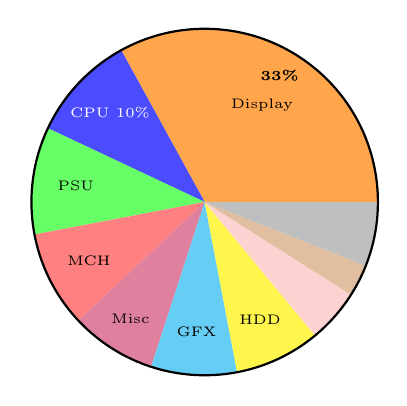
\begin{tikzpicture}[scale=1.1]
    % Pie chart - angles calculated from percentages (percent * 3.6)
    % Display 33%, CPU 10%, PSU 10%, MCH 9%, Misc 8%, GFX 8%, HDD 8%, CLK 5%, ICH 3%, Other 6%
    \def\radius{2}

    % Draw slices - cumulative angles
    % Display: 0 to 118.8 (33%)
    \fill[orange!70] (0,0) -- (0:\radius) arc (0:118.8:\radius) -- cycle;
    \node[font=\tiny] at (59.4:1.3) {Display};
    \node[font=\tiny\bfseries] at (59.4:1.7) {33\%};

    % CPU: 118.8 to 154.8 (10%)
    \fill[blue!70] (0,0) -- (118.8:\radius) arc (118.8:154.8:\radius) -- cycle;
    \node[font=\tiny, white] at (136.8:1.5) {CPU 10\%};

    % PSU: 154.8 to 190.8 (10%)
    \fill[green!60] (0,0) -- (154.8:\radius) arc (154.8:190.8:\radius) -- cycle;
    \node[font=\tiny] at (172.8:1.5) {PSU};

    % MCH: 190.8 to 223.2 (9%)
    \fill[red!50] (0,0) -- (190.8:\radius) arc (190.8:223.2:\radius) -- cycle;
    \node[font=\tiny] at (207:1.5) {MCH};

    % Misc: 223.2 to 252 (8%)
    \fill[purple!50] (0,0) -- (223.2:\radius) arc (223.2:252:\radius) -- cycle;
    \node[font=\tiny] at (237.6:1.6) {Misc};

    % GFX: 252 to 280.8 (8%)
    \fill[cyan!60] (0,0) -- (252:\radius) arc (252:280.8:\radius) -- cycle;
    \node[font=\tiny] at (266.4:1.5) {GFX};

    % HDD: 280.8 to 309.6 (8%)
    \fill[yellow!70] (0,0) -- (280.8:\radius) arc (280.8:309.6:\radius) -- cycle;
    \node[font=\tiny] at (295.2:1.5) {HDD};

    % CLK: 309.6 to 327.6 (5%)
    \fill[pink!70] (0,0) -- (309.6:\radius) arc (309.6:327.6:\radius) -- cycle;

    % ICH: 327.6 to 338.4 (3%)
    \fill[brown!50] (0,0) -- (327.6:\radius) arc (327.6:338.4:\radius) -- cycle;

    % Other: 338.4 to 360 (6%)
    \fill[gray!50] (0,0) -- (338.4:\radius) arc (338.4:360:\radius) -- cycle;

    % Draw outline
    \draw[thick] (0,0) circle (\radius);
\end{tikzpicture}
\end{center}
\end{column}
\begin{column}{0.45\textwidth}
\begin{itemize}
    \item \textbf{Display} dominates (33\%)
    \item CPU only 10\%
    \item Many fixed power consumers
    \item Optimizing CPU alone has limited impact
\end{itemize}
\end{column}
\end{columns}
\end{frame}

%% Slide: Smartphone Platform Power
\begin{frame}{Smartphone Platform Power}
\begin{columns}
\begin{column}{0.55\textwidth}
\begin{center}
\includegraphics[width=\textwidth]{figures/odpm.png}
\end{center}
\end{column}
\begin{column}{0.45\textwidth}
\textbf{Average power for 1-minute activities:}
\begin{itemize}
    \item YouTube 720p video
    \item Google Meet video call
    \item Instagram feed scrolling
    \item Clash of Clans gaming
    \item Idle standby
\end{itemize}

\vspace{2mm}
\begin{tcolorbox}[colback=yellow!10, colframe=orange!70, boxsep=1mm]
\small
\textbf{Cellular radio} often dominates power -- even more than display or CPU!
\end{tcolorbox}

\vspace{1mm}
{\tiny Gupta et al., ``3 W's of smartphone power consumption'', 2024}
\end{column}
\end{columns}
\end{frame}

%% Slide: Server Platform Power
\begin{frame}{Server Platform Power}
\begin{center}
\textbf{In servers, CPU dominates platform power}
\end{center}

\vspace{1mm}
\begin{columns}
\begin{column}{0.55\textwidth}
\begin{center}
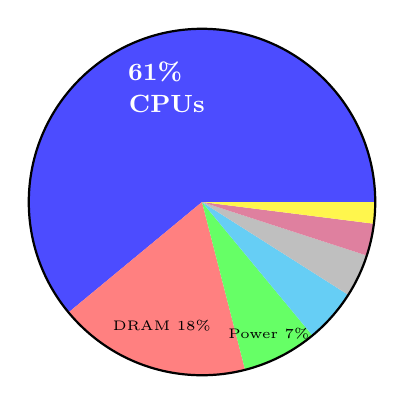
\begin{tikzpicture}[scale=1.1]
    \def\radius{2}

    % CPUs: 61% (0 to 219.6)
    \fill[blue!70] (0,0) -- (0:\radius) arc (0:219.6:\radius) -- cycle;
    \node[font=\small, white] at (109.8:1.2) {\textbf{CPUs}};
    \node[font=\small\bfseries, white] at (109.8:1.6) {61\%};

    % DRAM: 18% (219.6 to 284.4)
    \fill[red!50] (0,0) -- (219.6:\radius) arc (219.6:284.4:\radius) -- cycle;
    \node[font=\tiny] at (252:1.5) {DRAM 18\%};

    % Power overhead: 7% (284.4 to 309.6)
    \fill[green!60] (0,0) -- (284.4:\radius) arc (284.4:309.6:\radius) -- cycle;
    \node[font=\tiny] at (297:1.7) {Power 7\%};

    % Networking: 5% (309.6 to 327.6)
    \fill[cyan!60] (0,0) -- (309.6:\radius) arc (309.6:327.6:\radius) -- cycle;

    % Misc: 4% (327.6 to 342)
    \fill[gray!50] (0,0) -- (327.6:\radius) arc (327.6:342:\radius) -- cycle;

    % Cooling: 3% (342 to 352.8)
    \fill[purple!50] (0,0) -- (342:\radius) arc (342:352.8:\radius) -- cycle;

    % Storage: 2% (352.8 to 360)
    \fill[yellow!70] (0,0) -- (352.8:\radius) arc (352.8:360:\radius) -- cycle;

    % Draw outline
    \draw[thick] (0,0) circle (\radius);
\end{tikzpicture}
\end{center}
\end{column}
\begin{column}{0.45\textwidth}
\begin{itemize}
    \item \textbf{CPUs} dominate (61\%)
    \item DRAM significant (18\%)
    \item Power+cooling overhead (10\%)
    \item Storage, networking minimal
\end{itemize}

\vspace{2mm}
\begin{tcolorbox}[colback=blue!5, colframe=blue!50, boxsep=1mm]
\small
CPU optimization has major impact on server TCO!
\end{tcolorbox}

\vspace{1mm}
\hfill{\tiny Barroso et al., \textit{The Datacenter as a Computer}, 2018 (2017 servers)}
\end{column}
\end{columns}
\end{frame}

%% Slide: CPU Power Components
\begin{frame}{CPU Power Components}
\begin{columns}
\begin{column}{0.5\textwidth}
\textbf{Dynamic Power:} $P_{\text{dyn}} = C \cdot V^2 \cdot f$
\begin{itemize}
    \item $C$ -- capacitance of toggling transistors/wires
    \item $V$ -- voltage
    \item $f$ -- frequency
\end{itemize}

\textbf{Key insight:} $V \sim f$ $\Rightarrow$ $P \sim f^3$

\textbf{+X\% frequency $\Rightarrow$ $\sim$+3X\% power!}

\vspace{1mm}
\textbf{Leakage:} function of size, $V$, temp.
\end{column}
\begin{column}{0.5\textwidth}
\begin{tcolorbox}[colback=green!5, colframe=green!60, title={\small Example}, boxsep=1mm]
\footnotesize
$C = 1$nF, $V = 1$V, $f = 1$GHz, $P = 1$W\\[1mm]
$f$ increases 1\% to 1.01GHz\\
$V$ increases 1\% to 1.01V\\[1mm]
$P = 1.01^2 \times 1.01 = 1.03$W\\
\textbf{Power increases $\sim$3\%!}
\end{tcolorbox}

\begin{center}
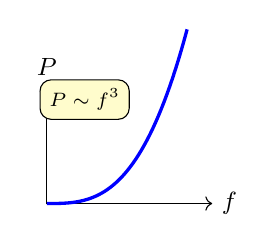
\begin{tikzpicture}[scale=0.6]
    \draw[->] (0,0) -- (3.5,0) node[right] {\small $f$};
    \draw[->] (0,0) -- (0,2.5) node[above] {\small $P$};
    \draw[blue, very thick, domain=0:1.35, samples=50] plot (\x*2.2, {(\x)^3 * 1.5});
    \node[draw, fill=yellow!20, rounded corners, font=\scriptsize,
          callout absolute pointer={(2.5, 1.5)}] at (0.8, 2.2) {$P \sim f^3$};
\end{tikzpicture}
\end{center}
\end{column}
\end{columns}
\end{frame}

%% Slide: Performance per Watt
\begin{frame}{Performance per Watt}
\small
\textbf{Goal:} Maximum performance at given power envelope (laptops, servers)

\vspace{2mm}
\textbf{When adding a new feature to increase IPC by Y\%:}
\begin{enumerate}
    \item New hardware adds power (dynamic + leakage)
    \item Added IPC causes entire core to toggle more (increases $C_{\text{dyn}}$)
\end{enumerate}

\vspace{2mm}
\begin{tcolorbox}[colback=red!5, colframe=red!60, boxsep=1mm]
\small
If feature increases $C$ by X\%, for fixed power must reduce frequency by $\frac{X}{3}$\%\\[1mm]
\textbf{Net performance gain} $\approx$ Y\% $-$ $\frac{X}{3}$\%\\[1mm]
$C_{\text{dyn}}$:IPC ratio -- if $\geq 3$ $\Rightarrow$ \textbf{net performance loss!}
\end{tcolorbox}

At $V_{\text{min}}$: if $C_{\text{dyn}}$:IPC $\geq 1$ $\Rightarrow$ loss
\end{frame}

%% Slide: Energy Efficiency
\begin{frame}{Energy Efficiency}
\[
E_{\text{active}} = P_{\text{active}} \times T_{\text{active}} \approx \frac{P_{\text{active}}}{\text{Perf}_{\text{active}}}
\]

\vspace{3mm}
\begin{columns}
\begin{column}{0.5\textwidth}
\textbf{Energy-efficient feature:}\\
1:1 performance : power ratio

\vspace{4mm}
\textbf{Most energy-efficient work point:}\\
Maximum frequency at $V_{\text{min}}$

\vspace{2mm}
Above that frequency: need to increase $V$ as well
\end{column}
\begin{column}{0.5\textwidth}
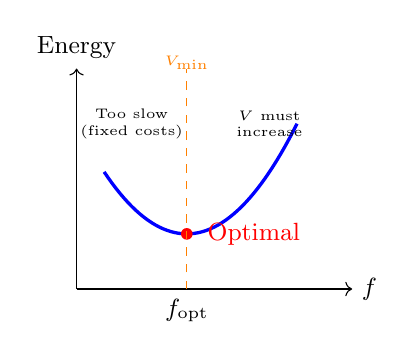
\begin{tikzpicture}[scale=0.7]
    \draw[->] (0,0) -- (5,0) node[right] {\small $f$};
    \draw[->] (0,0) -- (0,4) node[above] {\small Energy};

    % Energy curve (U-shaped)
    \draw[blue, very thick, domain=0.5:4, samples=50]
        plot (\x, {0.5*(\x-2)^2 + 1});

    % Mark optimal point
    \fill[red] (2, 1) circle (3pt);
    \node[below, font=\small] at (2, 0) {$f_{\text{opt}}$};
    \node[right, font=\small, red] at (2.2, 1) {Optimal};

    % Vmin line
    \draw[dashed, orange] (2, 0) -- (2, 4);
    \node[above, font=\tiny, orange] at (2, 3.8) {$V_{\text{min}}$};

    % Annotations
    \node[font=\tiny, align=center] at (1, 3) {Too slow\\(fixed costs)};
    \node[font=\tiny, align=center] at (3.5, 3) {$V$ must\\increase};
\end{tikzpicture}
\end{column}
\end{columns}
\end{frame}

\section{Power Management}

%% Slide: Managing Power Overview
\begin{frame}{Managing Power}
\begin{center}
\textbf{Typical CPU usage varies over time}

\vspace{2mm}
Bursts of high utilization \& long idle periods ($\sim$90\% idle for client)
\end{center}

\vspace{2mm}
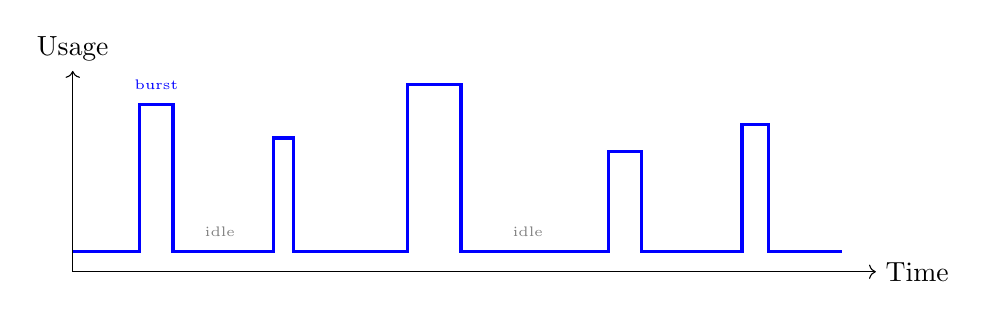
\begin{tikzpicture}[scale=0.85]
    \draw[->] (0,0) -- (12,0) node[right] {Time};
    \draw[->] (0,0) -- (0,3) node[above] {Usage};

    % Usage pattern
    \draw[blue, very thick]
        (0,0.3) -- (1,0.3) -- (1,2.5) -- (1.5,2.5) -- (1.5,0.3) --
        (3,0.3) -- (3,2) -- (3.3,2) -- (3.3,0.3) --
        (5,0.3) -- (5,2.8) -- (5.8,2.8) -- (5.8,0.3) --
        (8,0.3) -- (8,1.8) -- (8.5,1.8) -- (8.5,0.3) --
        (10,0.3) -- (10,2.2) -- (10.4,2.2) -- (10.4,0.3) -- (11.5,0.3);

    % Labels
    \node[font=\tiny, blue] at (1.25, 2.8) {burst};
    \node[font=\tiny, gray] at (2.2, 0.6) {idle};
    \node[font=\tiny, gray] at (6.8, 0.6) {idle};
\end{tikzpicture}

\vspace{2mm}
\textbf{Goal:} High power when needed; low power at idle
\end{frame}

%% Slide: P-States (DVFS)
\begin{frame}{Managing Power: P-States (DVFS)}
\small
\begin{columns}
\begin{column}{0.55\textwidth}
\textbf{Multiple voltage/frequency operating points}\\
OS changes frequency based on performance needs

\vspace{1mm}
\textbf{P-States:} P0 (max freq) $\rightarrow$ Pn ($V_{\text{min}}$, energy efficient)

\vspace{1mm}
\textbf{DVFS} = Dynamic Voltage and Frequency Scaling

$P = CV^2f$; $f = kV$ $\Rightarrow$ $P \sim f^3$, $E \sim f^2$
\end{column}
\begin{column}{0.45\textwidth}
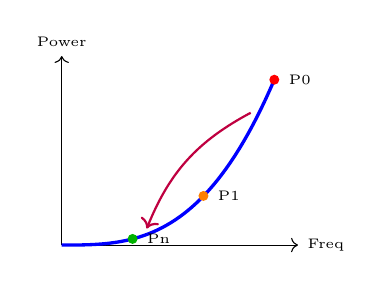
\begin{tikzpicture}[scale=0.6]
    \draw[->] (0,0) -- (5,0) node[right] {\tiny Freq};
    \draw[->] (0,0) -- (0,4) node[above] {\tiny Power};

    % Cubic curve P = k*f^3, with k chosen so curve passes through (4.5, 3.5)
    % k = 3.5/4.5^3 = 0.0384, so y = 0.0384 * x^3
    \draw[blue, very thick, domain=0:4.5, samples=50]
        plot (\x, {0.0384*(\x)^3});

    % P-state points ON the curve
    \fill[red] (4.5, 3.5) circle (3pt);
    \node[right, font=\tiny] at (4.6, 3.5) {P0};

    \fill[orange] (3, 1.04) circle (3pt);
    \node[right, font=\tiny] at (3.1, 1.04) {P1};

    \fill[green!70!black] (1.5, 0.13) circle (3pt);
    \node[right, font=\tiny] at (1.6, 0.13) {Pn};

    \draw[->, thick, purple] (4, 2.8) to[bend right=20] (1.8, 0.35);
\end{tikzpicture}

\begin{tcolorbox}[colback=green!5, colframe=green!50, boxsep=0.5mm]
\footnotesize
Small $f$ reduction $\Rightarrow$ Large $P$ savings
\end{tcolorbox}
\end{column}
\end{columns}
\end{frame}

%% Slide: C-States Overview
\begin{frame}{Managing Power: C-States (Sleep States)}
\begin{itemize}
    \item OS notifies CPU when no tasks are ready (using \texttt{MWAIT} instruction)
    \item CPU enters \textbf{sleep state} (C-state)
    \item \textbf{Tradeoff:} Deeper sleep $\Rightarrow$ more power savings, longer wakeup
\end{itemize}

\vspace{4mm}
\begin{center}
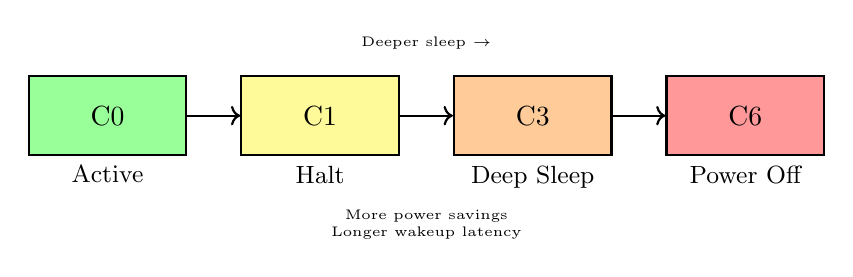
\begin{tikzpicture}[scale=0.9]
    % C-state boxes
    \node[draw, thick, fill=green!40, minimum width=2cm, minimum height=1cm] (c0) at (0,0) {C0};
    \node[draw, thick, fill=yellow!40, minimum width=2cm, minimum height=1cm] (c1) at (3,0) {C1};
    \node[draw, thick, fill=orange!40, minimum width=2cm, minimum height=1cm] (c3) at (6,0) {C3};
    \node[draw, thick, fill=red!40, minimum width=2cm, minimum height=1cm] (c6) at (9,0) {C6};

    \node[below, font=\small] at (c0.south) {Active};
    \node[below, font=\small] at (c1.south) {Halt};
    \node[below, font=\small] at (c3.south) {Deep Sleep};
    \node[below, font=\small] at (c6.south) {Power Off};

    % Arrows
    \draw[->, thick] (c0) -- (c1);
    \draw[->, thick] (c1) -- (c3);
    \draw[->, thick] (c3) -- (c6);

    % Labels
    \node[above, font=\tiny] at (4.5, 0.8) {Deeper sleep $\rightarrow$};
    \node[below, font=\tiny, align=center] at (4.5, -1.2) {More power savings\\Longer wakeup latency};
\end{tikzpicture}
\end{center}
\end{frame}

%% Slide: C-State Power Table
\begin{frame}{C-State Power (Intel Skylake-SP Server)}
\small
\begin{center}
\begin{tabular}{llccc}
\toprule
\rowcolor{gray!30} \textbf{C-State} & \textbf{Description} & \textbf{Transition} & \textbf{Target} & \textbf{Power/} \\
\rowcolor{gray!30} & & \textbf{time} & \textbf{residency} & \textbf{core} \\
\midrule
C0 (P1) & Active, base freq & --- & --- & $\sim$4 W \\
C0 (Pn) & Active, $V_{\text{min}}$ freq & --- & --- & $\sim$1 W \\
\rowcolor{yellow!20} C1 (P1) & Clock-gated (halt) & 2 $\mu$s & 2 $\mu$s & 1.44 W \\
\rowcolor{yellow!20} C1E (Pn) & Clock-gated + $V_{\text{min}}$ & 10 $\mu$s & 20 $\mu$s & 0.88 W \\
\rowcolor{orange!20} C6 & Power-gated, caches flushed & 133 $\mu$s & 600 $\mu$s & $\sim$0.1 W \\
\bottomrule
\end{tabular}
\end{center}

\vspace{2mm}
\begin{columns}
\begin{column}{0.55\textwidth}
\footnotesize
\textbf{Key observations:}
\begin{itemize}
    \item C6 saves $\sim$40$\times$ power vs C0
    \item 600$\mu$s residency to amortize transition
    \item C1E: good balance for short idle periods
\end{itemize}
\end{column}
\begin{column}{0.45\textwidth}
\begin{tcolorbox}[colback=blue!5, colframe=blue!50, boxsep=1mm]
\footnotesize
\textbf{Target residency}: min.\ time in state to justify transition energy
\end{tcolorbox}
\end{column}
\end{columns}

\hfill{\tiny Haj-Yahya et al., ``AgileWatts'', MICRO 2022}
\end{frame}

%% Slide: Putting it Together - Animation 1
\begin{frame}{Putting it Together: P-States and C-States}
\begin{center}
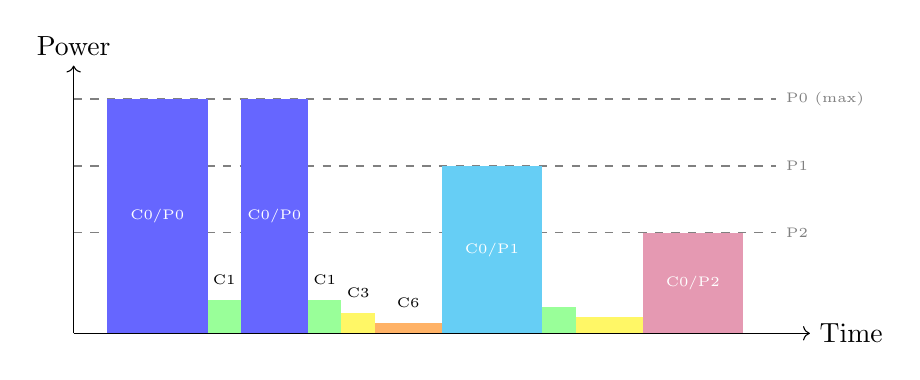
\begin{tikzpicture}[scale=0.85]
    \draw[->] (0,0) -- (11,0) node[right] {Time};
    \draw[->] (0,0) -- (0,4) node[above] {Power};

    % Power levels
    \draw[dashed, gray] (0, 3.5) -- (10.5, 3.5) node[right, font=\tiny] {P0 (max)};
    \draw[dashed, gray] (0, 2.5) -- (10.5, 2.5) node[right, font=\tiny] {P1};
    \draw[dashed, gray] (0, 1.5) -- (10.5, 1.5) node[right, font=\tiny] {P2};

    % Active periods at P0
    \fill[blue!60] (0.5, 0) rectangle (2, 3.5);
    \node[white, font=\tiny] at (1.25, 1.75) {C0/P0};

    % C1 dip
    \fill[green!40] (2, 0) rectangle (2.5, 0.5);
    \node[font=\tiny] at (2.25, 0.8) {C1};

    % Back to P0
    \fill[blue!60] (2.5, 0) rectangle (3.5, 3.5);
    \node[white, font=\tiny] at (3, 1.75) {C0/P0};

    % Longer idle - deeper C-states
    \fill[green!40] (3.5, 0) rectangle (4, 0.5);
    \fill[yellow!60] (4, 0) rectangle (4.5, 0.3);
    \fill[orange!60] (4.5, 0) rectangle (5.5, 0.15);
    \node[font=\tiny] at (3.75, 0.8) {C1};
    \node[font=\tiny] at (4.25, 0.6) {C3};
    \node[font=\tiny] at (5, 0.45) {C6};

    % Lower P-state operation
    \fill[cyan!60] (5.5, 0) rectangle (7, 2.5);
    \node[white, font=\tiny] at (6.25, 1.25) {C0/P1};

    % More idle
    \fill[green!40] (7, 0) rectangle (7.5, 0.4);
    \fill[yellow!60] (7.5, 0) rectangle (8.5, 0.25);

    % Even lower P-state
    \fill[purple!40] (8.5, 0) rectangle (10, 1.5);
    \node[white, font=\tiny] at (9.25, 0.75) {C0/P2};
\end{tikzpicture}
\end{center}

\vspace{2mm}
\begin{itemize}
    \item OS tracks CPU utilization history
    \item Switches to lower P-state when low activity detected
    \item Enters deeper C-states during idle periods
\end{itemize}
\end{frame}

%% Slide: Turbo Mode
\begin{frame}{Turbo Mode}
\begin{columns}
\begin{column}{0.55\textwidth}
\textbf{Without Turbo:}
\begin{itemize}
    \item All cores run at same frequency
    \item Frequency limited by TDP
\end{itemize}

\vspace{2mm}
\textbf{With Turbo Mode:}
\begin{itemize}
    \item Cores without threads $\rightarrow$ deep C-state (power gated)
    \item Use thermal budget of \textbf{idle} cores
    \item Boost frequency of \textbf{active} cores
\end{itemize}

\vspace{2mm}
\small
\textbf{Two turbo levels:}
\begin{itemize}
    \item \textbf{Guaranteed:} based on \# active cores
    \item \textbf{Opportunistic:} if thermal/power headroom
\end{itemize}
\end{column}
\begin{column}{0.45\textwidth}
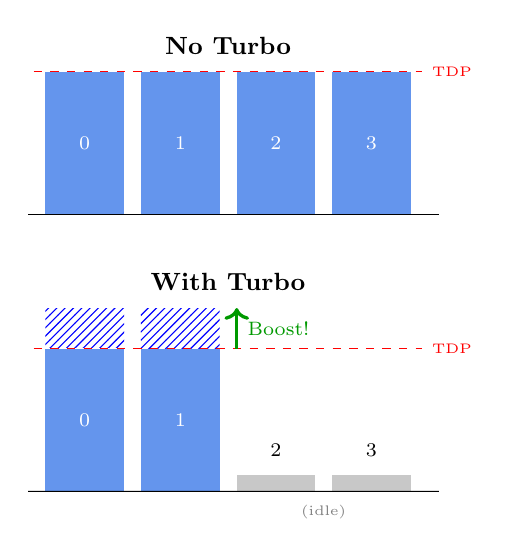
\begin{tikzpicture}[scale=0.7,
    % Styles
    core/.style={fill=corecolor, minimum width=1cm, minimum height=1.8cm, inner sep=0, anchor=south west},
    boost part/.style={fill=corecolor!70, pattern=north east lines, pattern color=blue, minimum width=1cm, minimum height=4mm, inner sep=0, anchor=south west},
    idle core/.style={fill=idlecolor, minimum width=1cm, minimum height=0.2cm, inner sep=0, anchor=south west},
    core label/.style={white, font=\scriptsize},
    section title/.style={font=\small\bfseries},
    tdp line/.style={dashed, red},
    tdp label/.style={font=\tiny, red},
    core gap/.style={xshift=2mm},
]
    % === No Turbo Section ===
    % Draw 4 equal cores - each relative to previous with gap
    \node[core] (nt-core-0) at (0, 0) {};
    \node[core, core gap] (nt-core-1) at (nt-core-0.south east) {};
    \node[core, core gap] (nt-core-2) at (nt-core-1.south east) {};
    \node[core, core gap] (nt-core-3) at (nt-core-2.south east) {};
    \node[core label] at (nt-core-0) {0};
    \node[core label] at (nt-core-1) {1};
    \node[core label] at (nt-core-2) {2};
    \node[core label] at (nt-core-3) {3};

    % Section title centered above all cores (close to bars)
    \node[section title, above=1mm of $(nt-core-1.north)!0.5!(nt-core-2.north)$] (no-turbo-title) {No Turbo};

    % TDP line at top of cores
    \draw[tdp line] ([xshift=-2mm]nt-core-0.north west) -- ([xshift=2mm]nt-core-3.north east)
        node[tdp label, right] {TDP};

    % X-axis for No Turbo section
    \draw ([xshift=-3mm]nt-core-0.south west) -- ([xshift=5mm]nt-core-3.south east);

    % === With Turbo Section ===
    % Base cores 0,1 (same height as No Turbo) - positioned below first section
    \node[core, below=17mm of nt-core-0.south west, anchor=north west] (t-core-0) {};
    \node[core, core gap] (t-core-1) at (t-core-0.south east) {};
    \node[core label] at (t-core-0) {0};
    \node[core label] at (t-core-1) {1};

    % Boost portions on top (with pattern) - positioned at north west of base cores
    \node[boost part, minimum height=0.5cm] (boost-0) at (t-core-0.north west) {};
    \node[boost part, minimum height=0.5cm] (boost-1) at (t-core-1.north west) {};

    % Idle cores 2,3 (power gated - flat) - same bottom alignment
    \node[idle core, core gap] (t-core-2) at (t-core-1.south east) {};
    \node[idle core, core gap] (t-core-3) at (t-core-2.south east) {};
    \node[font=\scriptsize, above=1mm of t-core-2] {2};
    \node[font=\scriptsize, above=1mm of t-core-3] {3};
    \node[font=\tiny, gray, below=0.5mm of $(t-core-2.south)!0.5!(t-core-3.south)$] {(idle)};

    % Section title at same x as "No Turbo", above boosted cores
    \node[section title] at (no-turbo-title |- boost-0.north) [above=1mm] {With Turbo};

    % TDP line at top of base cores (same as No Turbo height)
    \draw[tdp line] ([xshift=-2mm]t-core-0.north west) -- ([xshift=2mm]t-core-3.south east |- t-core-0.north)
        node[tdp label, right] {TDP};

    % X-axis for With Turbo section
    \draw ([xshift=-3mm]t-core-0.south west) -- ([xshift=5mm]t-core-3.south east);

    % Boost arrow relative to boost bar (xshift from south east to north east)
    \draw[->, green!60!black, very thick]
        ([xshift=3mm]boost-1.south east) -- ([xshift=3mm]boost-1.north east)
        node[right, font=\scriptsize, green!60!black, midway] {Boost!};
\end{tikzpicture}
\end{column}
\end{columns}
\end{frame}

%% Slide: Core and Graphics Power Budgeting
\begin{frame}{Core and Graphics Power Budgeting}
\begin{columns}
\begin{column}{0.5\textwidth}
\begin{itemize}
    \item Cores and Graphics on same die
    \item Separate voltage/frequency controls
    \item Tight HW control
    \item \textbf{Power budget can shift} between cores and graphics
\end{itemize}

\vspace{3mm}
Sum of max power $>$ Total package power\\
(realistic concurrent max is lower)
\end{column}
\begin{column}{0.5\textwidth}
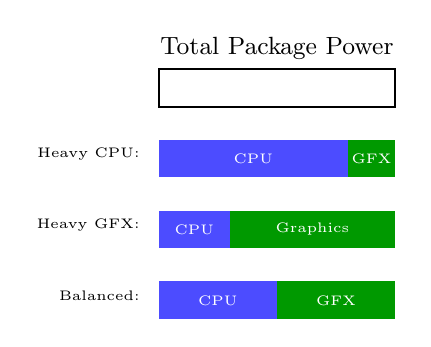
\begin{tikzpicture}[scale=0.6]
    % Total budget bar
    \draw[thick] (0, 0) rectangle (5, 0.8);
    \node[above, font=\small] at (2.5, 0.8) {Total Package Power};

    % Heavy CPU scenario
    \node[font=\tiny, left] at (-0.2, -1) {Heavy CPU:};
    \fill[blue!70] (0, -1.5) rectangle (4, -0.7);
    \fill[green!60!black] (4, -1.5) rectangle (5, -0.7);
    \node[white, font=\tiny] at (2, -1.1) {CPU};
    \node[white, font=\tiny] at (4.5, -1.1) {GFX};

    % Heavy GFX scenario
    \node[font=\tiny, left] at (-0.2, -2.5) {Heavy GFX:};
    \fill[blue!70] (0, -3) rectangle (1.5, -2.2);
    \fill[green!60!black] (1.5, -3) rectangle (5, -2.2);
    \node[white, font=\tiny] at (0.75, -2.6) {CPU};
    \node[white, font=\tiny] at (3.25, -2.6) {Graphics};

    % Balanced
    \node[font=\tiny, left] at (-0.2, -4) {Balanced:};
    \fill[blue!70] (0, -4.5) rectangle (2.5, -3.7);
    \fill[green!60!black] (2.5, -4.5) rectangle (5, -3.7);
    \node[white, font=\tiny] at (1.25, -4.1) {CPU};
    \node[white, font=\tiny] at (3.75, -4.1) {GFX};
\end{tikzpicture}
\end{column}
\end{columns}
\end{frame}

\section{Heterogeneous and Multi-Core}

%% Slide: Heterogeneous Processors
\begin{frame}{Heterogeneous Processors}
\begin{columns}
\begin{column}{0.55\textwidth}
\textbf{Combining ``big'' and ``small'' cores}

\vspace{3mm}
\textbf{Big cores:}
\begin{itemize}
    \item High-performance, high-power
    \item For demanding compute tasks
    \item Excel on single-threaded workloads
\end{itemize}

\vspace{2mm}
\textbf{Small cores:}
\begin{itemize}
    \item Energy-efficient
    \item Excel on low QoS workloads
    \item Many small cores = efficient multi-threaded
\end{itemize}

\vspace{3mm}
\textbf{ISA compatible} between big and small\\
$\Rightarrow$ Threads can migrate between core types
\end{column}
\begin{column}{0.45\textwidth}
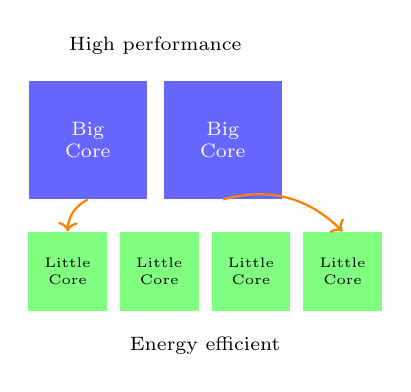
\begin{tikzpicture}[scale=0.7,
    % Styles
    big core/.style={fill=blue!60, minimum size=1.5cm, inner sep=1mm, align=center, font=\scriptsize, text=white},
    little core/.style={fill=green!50, minimum size=1cm, inner sep=0.5mm, align=center, font=\tiny},
    section label/.style={font=\scriptsize},
]
    % Big cores - first one anchored, second relative to first
    \node[big core] (big0) {Big\\Core};
    \node[big core, right=2mm of big0] (big1) {Big\\Core};

    % Fit node to get big row bounds
    \node[fit=(big0)(big1), inner sep=0] (big row) {};

    % Little cores - build row, then position via fit node
    \node[little core, below right=4mm and 0mm of big row.south west, anchor=north west] (little0) {Little\\Core};
    \node[little core, right=1.5mm of little0] (little1) {Little\\Core};
    \node[little core, right=1.5mm of little1] (little2) {Little\\Core};
    \node[little core, right=1.5mm of little2] (little3) {Little\\Core};

    % Fit node for little row
    \node[fit=(little0)(little3), inner sep=0] (little row) {};

    % Labels - positioned relative to fit nodes
    \node[section label, above=2mm of big row.north] {High performance};
    \node[section label, below=2mm of little row.south] {Energy efficient};

    % Migration arrows - using node anchors
    \draw[->, thick, orange] (big0.south) to[bend right=30] (little0.north);
    \draw[->, thick, orange] (big1.south) to[bend left=30] (little3.north);
\end{tikzpicture}

\vspace{3mm}
\begin{tcolorbox}[colback=gray!10, boxsep=1mm]
\small
Example: ARM big.LITTLE (2011)\\
Cortex-A15 (big) + Cortex-A7 (little)
\end{tcolorbox}
\end{column}
\end{columns}
\end{frame}

%% Slide: Heterogeneous Processor Scheduling
\begin{frame}{Heterogeneous Processor: Scheduling Approaches}
\begin{center}
\begin{tikzpicture}[
    % Core styles
    big core/.style={fill=blue!50, minimum width=8mm, minimum height=10mm},
    little core/.style={fill=green!50, minimum width=6mm, minimum height=7mm},
    % Title style
    approach title/.style={font=\small\bfseries, anchor=south},
    % Description style
    desc/.style={font=\scriptsize, text width=3cm, align=center, anchor=north},
    % Cluster box style
    cluster box/.style={draw, thick, dashed, rounded corners=2pt, inner sep=1.5mm},
    % Callout base style (pointer set per-node)
    callout base/.style={rectangle callout, draw, fill=yellow!20, font=\scriptsize,
                    text width=2.8cm, align=left, rounded corners=1pt},
]
    % === Column positions (spread wider) ===
    \coordinate (col1) at (0, 0);
    \coordinate (col2) at (4.5, 0);
    \coordinate (col3) at (9, 0);

    % ============ CLUSTERED SWITCHING ============
    % Big cores cluster
    \node[big core] (clust-big1) at ([yshift=10mm, xshift=-5mm]col1) {};
    \node[big core, right=1mm of clust-big1] (clust-big2) {};
    \node[fit=(clust-big1)(clust-big2), cluster box, red] (clust-big-box) {};
    \node[fit=(clust-big1)(clust-big2), inner sep=0] (clust-bigs) {};  % for title positioning

    % Little cores cluster
    \node[little core] (clust-lit1) at ([yshift=-6mm, xshift=-4mm]col1) {};
    \node[little core, right=1mm of clust-lit1] (clust-lit2) {};
    \node[fit=(clust-lit1)(clust-lit2), cluster box, red] (clust-lit-box) {};

    % OR label
    \node[font=\scriptsize, red] (clust-or) at ($(clust-big-box.south)!0.5!(clust-lit-box.north)$) {OR};

    % Title - use inner sep=0 fit node for consistent positioning
    \node[approach title, above=2mm of clust-bigs.north] {Clustered Switching};

    % Description
    \node[desc] at ([yshift=-15mm]col1) {OS sees one cluster. Switch entire cluster based on load.};

    % ============ IN-KERNEL SWITCHING ============
    % Virtual core 1 - big core at same level as clustered big cores
    \node[big core] (inker-big1) at ([yshift=10mm, xshift=-9mm]col2) {};
    % Little core aligned with clustered little cores y-position
    \node[little core] (inker-lit1) at (inker-big1 |- clust-lit1) {};
    \node[fit=(inker-big1)(inker-lit1), cluster box, orange, inner sep=1mm] (inker-vcore1) {};
    \node[font=\scriptsize, orange] at ($(inker-big1.south)!0.5!(inker-lit1.north)$) {OR};
    \node[font=\tiny, below=-0.5mm of inker-vcore1, anchor=north] {vCore1};

    % Virtual core 2
    \node[big core] (inker-big2) at ([yshift=10mm, xshift=9mm]col2) {};
    \node[little core] (inker-lit2) at (inker-big2 |- clust-lit1) {};
    \node[fit=(inker-big2)(inker-lit2), cluster box, orange, inner sep=1mm] (inker-vcore2) {};
    \node[font=\scriptsize, orange] at ($(inker-big2.south)!0.5!(inker-lit2.north)$) {OR};
    \node[font=\tiny, below=-0.5mm of inker-vcore2, anchor=north] {vCore2};

    % Title - use fit node spanning both big cores for consistent positioning
    \node[fit=(inker-big1)(inker-big2), inner sep=0] (inker-bigs) {};
    \node[approach title, above=2mm of inker-bigs.north] {In-Kernel Switching};

    % Fit node for both vcores (for callout pointer)
    \node[fit=(inker-vcore1)(inker-vcore2), inner sep=0] (inker-vcores) {};

    % Description
    \node[desc] at ([yshift=-15mm]col2) {Paired big+little form virtual cores. One active per pair.};

    % ============ GLOBAL SCHEDULING ============
    % Big cores row
    \node[big core] (glob-big1) at ([yshift=10mm, xshift=-5mm]col3) {};
    \node[big core, right=1mm of glob-big1] (glob-big2) {};

    % Little cores row - aligned with clustered little cores
    \node[little core] (glob-lit1) at ([xshift=-10mm]col3 |- clust-lit1) {};
    \node[little core, right=1mm of glob-lit1] (glob-lit2) {};
    \node[little core, right=1mm of glob-lit2] (glob-lit3) {};
    \node[little core, right=1mm of glob-lit3] (glob-lit4) {};

    % Fit node for all global cores (for callout pointer)
    \node[fit=(glob-big1)(glob-big2)(glob-lit1)(glob-lit4), inner sep=0] (glob-all) {};

    % Title - close to illustration
    \node[fit=(glob-big1)(glob-big2), inner sep=0] (glob-bigs) {};
    \node[approach title, above=2mm of glob-bigs.north] {HMP};

    % Description
    \node[desc] at ([yshift=-15mm]col3) {Heterogeneous Multi-Processing. All cores visible.};

    % ============ FLEXIBILITY SCALE ============
    \coordinate (scale-y) at (0, -3.4);
    \draw[->, thick] ([xshift=-1.5cm]scale-y) -- ([xshift=10.5cm]scale-y);
    \node[font=\small, anchor=east] at ([xshift=-1.6cm]scale-y) {Simple};
    \node[font=\small, anchor=west] at ([xshift=10.6cm]scale-y) {Flexible};

    \fill (col1 |- scale-y) circle (2.5pt);
    \node[above=1mm, font=\tiny] at (col1 |- scale-y) {Clustered};
    \node[below=1mm, font=\tiny, gray, align=center] at (col1 |- scale-y) {Galaxy S4\\2013};

    \fill (col2 |- scale-y) circle (2.5pt);
    \node[above=1mm, font=\tiny] at (col2 |- scale-y) {In-Kernel};
    \node[below=1mm, font=\tiny, gray, align=center] at (col2 |- scale-y) {Galaxy S4\\w/ Linux};

    \fill (col3 |- scale-y) circle (2.5pt);
    \node[above=1mm, font=\tiny] at (col3 |- scale-y) {HMP};
    \node[below=1mm, font=\tiny, gray, align=center] at (col3 |- scale-y) {Galaxy S5+\\2014};

    % ============ CALLOUTS (one at a time using \only) ============
    % Clustered callout (overlay 2 only)
    \only<2>{
        \node[callout base, callout absolute pointer={(clust-or.east)}, anchor=west,
              text width=3.5cm]
            at ([xshift=5mm]clust-lit-box.east)
            {\textbf{Transparent} to OS\\[1pt]
             Hypervisor switches clusters;\\data passes through L2};
    }

    % In-Kernel callout (overlay 3 only) - positioned relative to right vcore
    \only<3>{
        \node[callout base, callout absolute pointer={(inker-vcore2.east)}, anchor=west,
              text width=3.5cm]
            at ([xshift=5mm]inker-vcore2.east)
            {\textbf{One core} active per pair\\[1pt]
             Can use existing DVFS interface (e.g., cpufreq)};
    }

    % HMP callout (overlay 4+) - left of leftmost small core
    \visible<4->{
        \node[callout base, callout absolute pointer={(glob-lit1.west)}, anchor=east,
              text width=3.2cm]
            at ([xshift=-5mm]glob-lit1.west)
            {\textbf{All cores} visible to OS\\[1pt]
             Direct task migration between any cores};
    }
\end{tikzpicture}
\end{center}
\end{frame}

%% Slide: Turbo Boost 2.0
\begin{frame}{Intel Turbo Boost Technology 2.0}
\footnotesize
\begin{columns}
\begin{column}{0.55\textwidth}
After idle, system accumulates ``energy budget'' to accommodate high power for short bursts. In steady state, power stabilizes at TDP.

\vspace{2mm}
\textbf{P-State ranges:}
\begin{itemize}
    \item \textbf{P1}: Guaranteed freq (worst case)
    \item \textbf{P0}: Max turbo freq
    \item \textbf{P1--P0}: HW controlled
    \item \textbf{Pn}: Energy efficient
\end{itemize}

OS treats P0 as any other P-state; P1 to P0 is HW controlled
\end{column}
\begin{column}{0.45\textwidth}
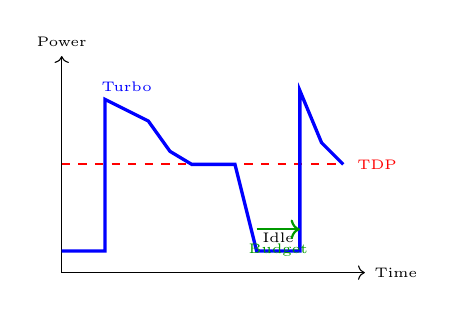
\begin{tikzpicture}[scale=0.55]
    \draw[->] (0,0) -- (7,0) node[right] {\tiny Time};
    \draw[->] (0,0) -- (0,5) node[above] {\tiny Power};

    % TDP line
    \draw[dashed, red, thick] (0, 2.5) -- (6.5, 2.5);
    \node[right, font=\tiny, red] at (6.6, 2.5) {TDP};

    % Power trace
    \draw[blue, very thick]
        (0, 0.5) -- (1, 0.5) -- (1, 4) -- (2, 3.5) -- (2.5, 2.8) -- (3, 2.5) --
        (4, 2.5) -- (4.5, 0.5) -- (5.5, 0.5) -- (5.5, 4.2) -- (6, 3) -- (6.5, 2.5);

    % Labels
    \node[font=\tiny, blue] at (1.5, 4.3) {Turbo};
    \node[font=\tiny] at (5, 0.8) {Idle};

    % Budget buildup
    \draw[->, green!60!black, thick] (4.5, 1) -- (5.5, 1);
    \node[font=\tiny, green!60!black, below] at (5, 0.9) {Budget};
\end{tikzpicture}

\vspace{1mm}
\colorbox{blue!10}{\parbox{0.95\linewidth}{\scriptsize Use accumulated budget to enhance responsiveness}}
\end{column}
\end{columns}
\end{frame}

%% Slide: CMP Performance vs Power
\begin{frame}{CMP: Performance vs Power}
\small
\begin{tcolorbox}[colback=yellow!10, colframe=orange!70, boxsep=1mm]
$2\times$ CPUs $\neq$ $2\times$ performance; $2\times$ CPUs $\Rightarrow$ $\frac{1}{2}$ power each
\end{tcolorbox}

\vspace{2mm}
\textbf{Example:} CPU at 3.8GHz for 100W. \textbf{Dual-core:} 50W per CPU

\vspace{1mm}
$P \sim V^3$: $\frac{V_{\text{orig}}^3}{V_{\text{CMP}}^3} = \frac{100}{50}$ $\Rightarrow$ $V_{\text{CMP}} = 0.8 V_{\text{orig}}$

$f \sim V$: $f_{\text{CMP}} = 0.8 \times 3.8 = 3.0$GHz

\vspace{2mm}
\textbf{Result:} 2 cores @ 3.0GHz vs 1 core @ 3.8GHz\\
Multi-threaded: $2 \times \frac{3.0}{3.8} = 1.58\times$ speedup (not $2\times$!)
\end{frame}

%% Slide: Example Problem
\begin{frame}{Example: Power/Performance Trade-off}
\footnotesize
\textbf{Problem:} Design MP system with 60W envelope ($\frac{2}{3}$ for cores = 40W)

\vspace{2mm}
\begin{center}
\begin{tabular}{lcc}
\toprule
\rowcolor{gray!30} & \textbf{Big Core} & \textbf{Small Core} \\
\midrule
Area & 4mm$^2$ & 2mm$^2$ \\
IPC & 3 & 2 \\
Freq @ $V_{\text{min}}=0.7$V & 1.35GHz & 1.45GHz \\
\bottomrule
\end{tabular}
\hspace{5mm}
\begin{tabular}{l}
\rowcolor{gray!30} \textbf{Given} \\
\midrule
Leakage: 0.25W/mm$^2$ \\
$C = \text{IPC} \times 750$pF \\
\\
\end{tabular}
\end{center}

\vspace{2mm}
\textbf{Power per core:} $P = C \cdot V^2 \cdot f + P_{\text{leak}}$
\begin{itemize}
    \item Big: $P = 2.25\text{nF} \times 0.49 \times 1.35 + 1\text{W} = 2.49$W \quad $\Rightarrow$ \textbf{16 cores} fit in 40W
    \item Small: $P = 1.5\text{nF} \times 0.49 \times 1.45 + 0.5\text{W} = 1.57$W \quad $\Rightarrow$ \textbf{25 cores} fit in 40W
\end{itemize}

\vspace{2mm}
\begin{tcolorbox}[colback=green!5, colframe=green!60, boxsep=1mm]
\textbf{Throughput:} Big: $16 \times 3 \times 1.35 = 64.8$ Ginst/s \quad Small: $25 \times 2 \times 1.45 = \mathbf{72.5}$ Ginst/s
\end{tcolorbox}
\end{frame}

%% Slide: Race to Halt vs Slow and Steady
\begin{frame}{Total Platform Energy: Race to Halt?}
\footnotesize
\begin{columns}
\begin{column}{0.5\textwidth}
Platform has fixed power components ($P_{\text{SYS}}$)

\vspace{1mm}
\textbf{Derivation} (for fixed work, $T \sim \frac{1}{f}$):
\begin{itemize}
    \item $P_{\text{CPU}} \sim f^3$ $\Rightarrow$ $E_{\text{CPU}} = P \times T \sim f^3 \times \frac{1}{f} = f^2$
    \item $P_{\text{SYS}} = K$ $\Rightarrow$ $E_{\text{SYS}} = K \times T \sim \frac{1}{f}$
\end{itemize}

\vspace{1mm}
\textbf{System-dominated:} \textbf{Race to Halt}\\
{\scriptsize (run fast $\rightarrow$ short $T$ $\rightarrow$ less $E_{\text{SYS}}$)}

\vspace{1mm}
\textbf{CPU-dominated:} \textbf{Lowest frequency}\\
{\scriptsize (slow $\rightarrow$ less $E_{\text{CPU}}$)}

\vspace{1mm}
$\Rightarrow$ Total energy has \textbf{optimal frequency}
\end{column}
\begin{column}{0.5\textwidth}
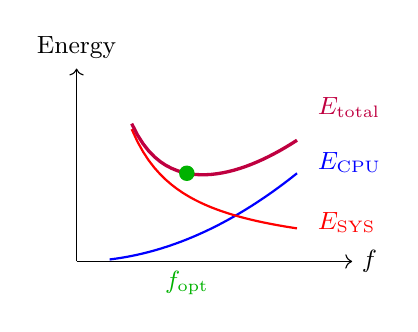
\begin{tikzpicture}[scale=0.7]
    \draw[->] (0,0) -- (5,0) node[right] {\small $f$};
    \draw[->] (0,0) -- (0,3.5) node[above] {\small Energy};

    % E_CPU ~ f^2
    \draw[blue, thick, domain=0.3:2, samples=30]
        plot (\x*2, {0.4*\x*\x});
    \node[blue, font=\small, right] at (4.2, 1.8) {$E_{\text{CPU}}$};

    % E_SYS ~ 1/f (displayed as fraction)
    \draw[red, thick, domain=0.5:2, samples=30]
        plot (\x*2, {1.2/\x});
    \node[red, font=\small, right] at (4.2, 0.7) {$E_{\text{SYS}}$};

    % Total
    \draw[purple, very thick, domain=0.5:2, samples=30]
        plot (\x*2, {0.4*\x*\x + 1.2/\x});
    \node[purple, font=\small, right] at (4.2, 2.8) {$E_{\text{total}}$};

    % Optimal point
    \fill[green!70!black] (2, 1.6) circle (4pt);
    \node[below, font=\small, green!70!black] at (2, 0) {$f_{\text{opt}}$};
\end{tikzpicture}

\vspace{1mm}
\textbf{Example:} $P_{\text{SYS}}=10$W, $P_{\text{CPU}}=4$W @ 2GHz

{\scriptsize
\begin{tabular}{lcc}
\rowcolor{gray!30} & \textbf{2GHz} & \textbf{1GHz} \\
$T$ & 1s & 2s \\
$E_{\text{CPU}}$ & 4J & 1J \\
$E_{\text{SYS}}$ & 10J & 20J \\
\textbf{Total} & \textbf{14J} & 21J \\
\end{tabular}
$\Rightarrow$ Race to Halt wins!
}
\end{column}
\end{columns}
\end{frame}

%% Slide: Summary
\begin{frame}{Summary}
\begin{columns}
\begin{column}{0.5\textwidth}
\textbf{Power Fundamentals:}
\begin{itemize}
    \item $P_{\text{dyn}} = CV^2f \sim f^3$
    \item TDP vs Average Power
    \item Performance per Watt
    \item Energy efficiency at $V_{\text{min}}$
\end{itemize}

\vspace{3mm}
\textbf{Power Management:}
\begin{itemize}
    \item P-States (DVFS)
    \item C-States (sleep)
    \item Turbo Mode
    \item Core/Graphics budgeting
\end{itemize}
\end{column}
\begin{column}{0.5\textwidth}
\textbf{Advanced Topics:}
\begin{itemize}
    \item Heterogeneous processors
    \item big.LITTLE architecture
    \item Scheduling approaches
    \item CMP power trade-offs
\end{itemize}

\vspace{3mm}
\begin{tcolorbox}[colback=green!10, colframe=green!60]
\textbf{Key Insight:}\\
Power management is about\\
\textbf{right power at right time}\\
High when needed, low otherwise
\end{tcolorbox}
\end{column}
\end{columns}
\end{frame}

\end{document}
